\appendix
\section{Supplementary material to Structured Recommendation}
\label{sec:supplement}

\subsection{1-slack formulation for the SR model}
\label{ssec:1slack_sr}

We can use \emph{one} slack variable to represent the sum of the $N$ hinge losses:
\begin{equation*}
%%\label{eq:hingeloss}
%%\resizebox{1.1\linewidth}{!}{
%%\begin{minipage}{\linewidth}
%\begin{align*}
\xi_i = \max \left( 0, \, 
        \max_{\bar{\y} \in \mathcal{Y}}
        \left\{ \Delta(\y^{(i)}, \bar{\y}) + \w^\top \Psi(\x^{(i)}, \bar{\y}) \right\} - \w^\top \Psi(\x^{(i)}, \y^{(i)}) \right).
%\end{align*}
%%\end{minipage}
%%}
\end{equation*}
Which results in the 1-slack formulation for the SR model:
\begin{equation*}
%%\label{eq:1slack_ml}
\resizebox{0.9\linewidth}{!}{$
\begin{aligned}
\min_{\w, \, \xi \ge 0} ~\frac{1}{2} \w^\top \w + C \xi, ~~s.t.~ \frac{1}{N} \left( \sum_{i,j} \w^\top \Psi(\x^{(i)}, \y^{(ij)}) - \w^\top \Psi(\x^{(i)}, \bar{\y}^{(i)}) \right) 
  \ge \frac{1}{N} \sum_{i,j} \Delta(\y^{(ij)}, \bar{\y}^{(i)}) - \xi.
\end{aligned}
$}
\end{equation*}


\subsection{The list Viterbi algorithm}
\label{sec:listviterbi-supp}

We make use of the list Viterbi in four situations:
\begin{enumerate}
  \item To avoid sequence with loops during the prediction phase of the SP and SR models
  \item To make top-$k$ prediction using the SP and SR models
  \item To eliminate known ground truths during the training phase (\ie loss augmented inference) of the SR and \textsc{SRpath} models
  \item To avoid sequence with loops during the training phase (\ie loss augmented inference) of the \textsc{SPpath} and \textsc{SRpath} models
\end{enumerate}

%%There are two general approaches for generalising Viterbi decoding to when we require $k$
%%sequences to be decoded: by maintaining $k$ paths through the trellis while decoding; or by
%%careful book keeping of the best $k-1$ paths through the trellis found so far and avoiding them.
%%We choose the latter approach as it is more memory efficient.

The serial list Viterbi algorithm~\cite{nilsson2001sequentially,seshadri1994list} maintains
a heap (\ie priority queue) of potential solutions, which are then checked for the desired property (for example
whether there are loops). Once the requisite number of trajectories with the desired
property are found, the algorithm terminates (for example once $k$ trajectories without loops are found when performing top-k prediction)
The heap is initialised by running forward-backward (Algorithm~\ref{alg:forward-backward}) followed by the vanilla Viterbi (Algorithm~\ref{alg:viterbi}).

\begin{algorithm}[htbp]
\caption{Forward-backward procedure~\cite{rabiner1989tutorial}}
\label{alg:forward-backward}
\begin{algorithmic}[1]
  \STATE $\forall p_j \in \mathcal{P},~ \alpha_t(p_j) =
          \begin{cases}
          0,~ t = 1 \\
          \max_{p_i \in \mathcal{P}} \left\{ \alpha_{t-1}(p_i) + \mathbf{w}_{ij}^\top \Psi_{ij}(\mathbf{x}, p_i, p_j) +
          \mathbf{w}_j^\top \Psi_j(\mathbf{x}, p_j) \right\},~ t=2,\dots,l
          \end{cases}$

  \STATE $\forall p_i \in \mathcal{P},~ \beta_t(p_i) =
          \begin{cases}
          0,~ t = l \\
          \max_{p_j \in \mathcal{P}} \left\{ \mathbf{w}_{ij}^\top \Psi_{ij}(\mathbf{x}, p_i, p_j) +
          \mathbf{w}_j^\top \Psi_j(\mathbf{x}, p_j) + \beta_{t+1}(p_j) \right\},~ t = l-1,\dots,1
          \end{cases}$

  %\STATE $\forall p_i \in \mathcal{P},~ f_t(p_i) = \alpha_t(p_i) + \beta_t(p_i),~ t = 1,\dots,K$
  \STATE $\forall p_i, p_j \in \mathcal{P},~ f_{t,t+1}(p_i, p_j) = \alpha_t(p_i) + \mathbf{w}_{ij}^\top \Psi_{ij}(\mathbf{x}, p_i, p_j) +
                                \mathbf{w}_j^\top \Psi_j(\mathbf{x}, p_j) + \beta_{t+1}(p_j),~ t = 1,\dots,l-1$
\end{algorithmic}
\end{algorithm}

\begin{algorithm}[htbp]
\caption{Viterbi}
\label{alg:viterbi}
\begin{algorithmic}[1]
  \STATE $y_t^1 = \begin{cases}
                  s,~ t = 1 \\
  %                \argmax_{p \in \mathcal{P}} \left\{ f_{1,2}(s, p) \right\},~ t = 2, \\
                  \argmax_{p \in \mathcal{P}} \left\{ f_{t-1,t}(y_{t-1}^1, p) \right\},~ t = 2,\dots,l
                  \end{cases}$

  %\STATE $r^1 = \max_{p \in \mathcal{P}} \left\{ f_K(p) \right\}~~~ \triangleright$ $r^1$ is the score/priority of $\mathbf{y}^1$
  \STATE $r^1 = \max_{p \in \mathcal{P}} \left\{ \alpha_{l}(p) \right\}~~~ \triangleright$ $r^1$ is the score/priority of $\mathbf{y}^1$
\end{algorithmic}
\end{algorithm}

Given an existing heap containing potential trajectories,
list Viterbi maintains a set of POIs $S$ to exclude, which is updated
sequentially by considering the front sequence of the heap.

Recall that for trajectory recommendation we are given the query $\mathbf{x}=(s, l)$, where
$s$ is the starting POI from the set of POIs $\mathcal{P}$,
and $l$ is the desired length of the trajectory.
We assume the score function is of the form $\mathbf{w}^\top \Psi$ where $\Psi$ is the joint
feature vector. $\mathbf{w}$ could be the value of the weight in the current iteration in training,
or the learned weight vector during prediction.

The list Viterbi algorithm for performing top-$k$ prediction is described in Algorithm~\ref{alg:listviterbi}.
To eliminating known ground truths in loss augmented inference,
we modify the forward-backward procedure (Algorithm~\ref{alg:forward-backward}) to account for the loss term $\Delta(\cdot,\cdot)$,
and Algorithm~\ref{alg:viterbi} and Algorithm~\ref{alg:listviterbi} can be used without modification.

\begin{algorithm}[htbp]
\caption{The list Viterbi algorithm for top-$K$ prediction~\cite{nilsson2001sequentially,seshadri1994list}}
\label{alg:listviterbi}
\begin{algorithmic}[1]
\STATE \textbf{Input}: $\mathbf{x}=(s, l),~ \mathcal{P},~ \mathbf{w},~ \Psi, ~K$
%\STATE Initialise score matrices $\alpha,~ \beta,~ f_t,~ f_{t, t+1}$, a max-heap $H,~ k=0$.
\STATE Initialise score matrices $\alpha,~ \beta,~ f_{t, t+1}$, a max-heap $H$, result set $R$, $k=0$.
\STATE $\triangleright$ Do the forward-backward procedure (Algorithm~\ref{alg:forward-backward})
\STATE $\triangleright$ Identify the best (scored) trajectory $\mathbf{y}^1=(y_1^1,\dots,y_l^1)$
  with Viterbi (Algorithm~\ref{alg:viterbi}). This may be a trajectory that violates the desired condition.
\STATE $H.\textit{push}\left(r^1,~ (\mathbf{y}^1, \textsc{nil}, \emptyset) \right)$
\STATE Set $R=\emptyset$, the list of trajectories to be returned.
\WHILE{$H \ne \emptyset$ \textbf{and} $k < \,|\mathcal{P}|^{l-1} - \prod_{t=2}^l (|\mathcal{P}|-t+1) + K$}
    \STATE $r^k,~ (\mathbf{y}^k, I, S) = H.\textit{pop}()~~~ \triangleright$
           $r^k$ is the score of $\mathbf{y}^k=(y_1^k,\dots,y_l^k)$, $I$ is the partition index, and $S$ is the exclude set
    \STATE $k = k + 1$
    \STATE Add $\mathbf{y}^k$ to $R$ if it satisfies the desired property
    \RETURN $R$ if it contains the required number of trajectories
    \STATE $\bar{I} = \begin{cases}
                      2,~ I = \textsc{nil} \\
                      I,~ \text{otherwise}
                      \end{cases}$

    \FOR{$t = \bar{I},\dots,l$}
        \STATE $\bar{S} = \begin{cases}
                          S \cup \{ y_t^k \},& t = \bar{I} \\
                          \{ y_t^k \},& \text{otherwise}
                          \end{cases}$

        \STATE $\bar{y}_j = \begin{cases}
                            y_j^k,& j=1,\dots,t-1 \\
                            %\argmax_{p \in \mathcal{P} \setminus \textit{new\_exclude\_set}} f_{t-1,t}(y_{t-1}^k, p),~ j=t \\
                            \argmax_{p \in \mathcal{P} \setminus \bar{S}} \left\{ f_{t-1,t}(y_{t-1}^k, p) \right\},& j=t \\
                            \argmax_{p \in \mathcal{P}} \left\{ f_{j-1, j}(\bar{y}_{j-1}, p) \right\},& j=t+1,\dots,l
                \end{cases}$
        \STATE $\bar{r} = \begin{cases}
                          f_{t-1,t}(y_{t-1}^k, \bar{y}_t),&I = \textsc{nil} \\
                          r^k + f_{t-1,t}(y_{t-1}^k, \bar{y}_t) - f_{t-1,t}(y_{t-1}^k, y_t^k), &\text{otherwise}
                          \end{cases}$

        $H.\textit{push}\left(\bar{r}, (\bar{\mathbf{y}}, t, \bar{S}) \right)$
    \ENDFOR
\ENDWHILE
\end{algorithmic}
\end{algorithm}

\clearpage
\subsection{Photo Trajectory Dataset and Features}
\label{sec:feature}

\textbf{Dataset}.
In the interests of reproducibility we present further details of our empirical experiment.
The histogram of the number of trajectories per query is shown in Figure~\ref{fig:hist_query},
where we can see each query has 4-9 ground truths (\ie trajectories) on average, and 30-60 trajectories at most.
The histogram of trajectory length (\ie the number of POIs in a trajectory) is shown in Figure~\ref{fig:hist_length},
where we can see the majority are short trajectories (\ie length $\le$ 5).

% histogram of #ground truth
\begin{figure}[t]
	\centering
	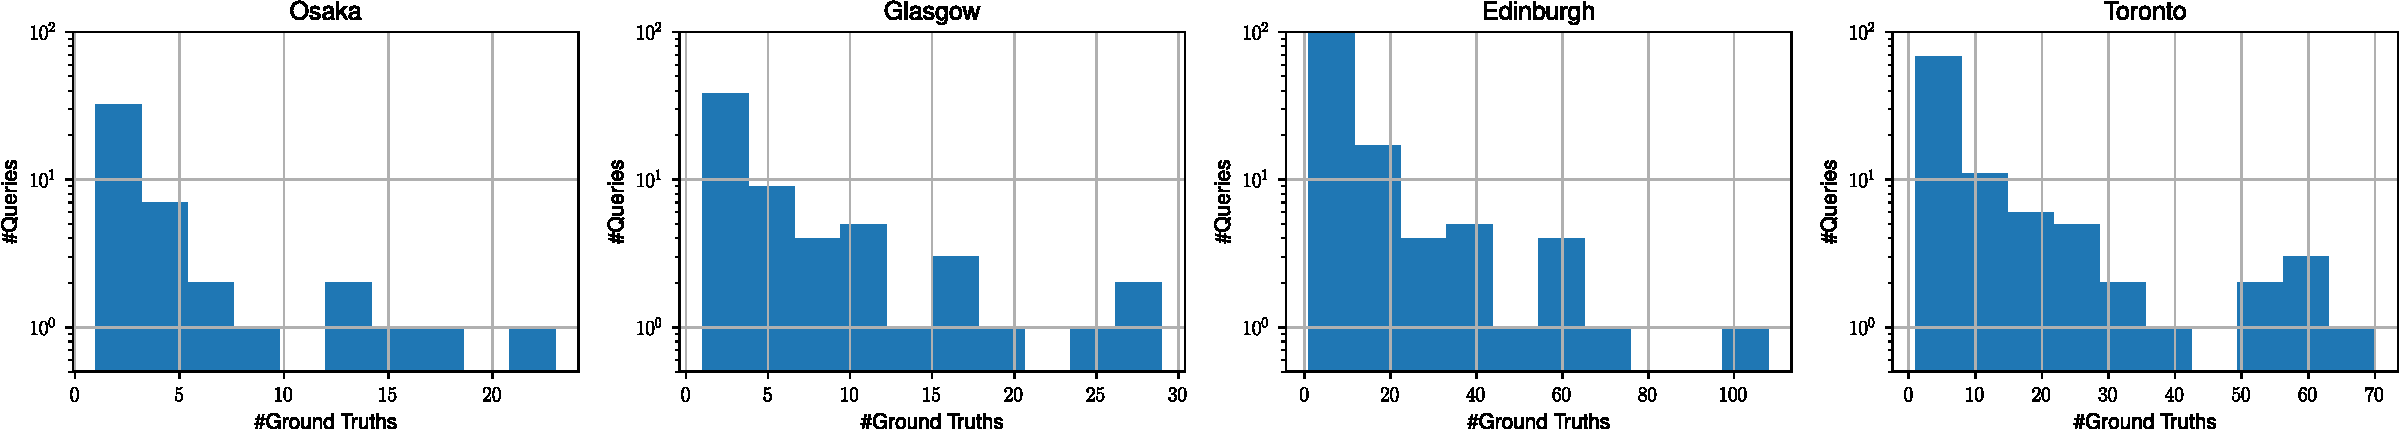
\includegraphics[width=.9\linewidth]{hist_query.pdf}
	\caption{Histograms of the number of trajectories per query.}
	\label{fig:hist_query}
\end{figure}


% histogram of trajectory length
\begin{figure}[t]
	\centering
	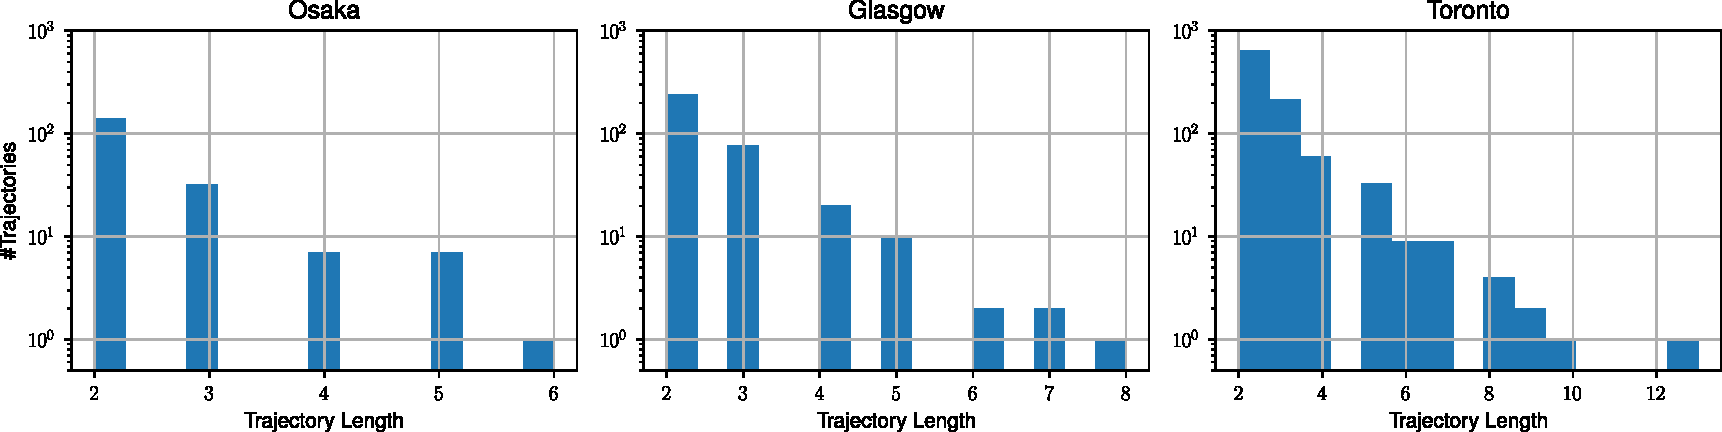
\includegraphics[width=.9\linewidth]{hist_length.pdf}
	\caption{Histograms of trajectory length.}
	\label{fig:hist_length}
\end{figure}


\textbf{Features}.
The POI-query features used by \textsc{PoiRank}, SP and SR methods and their extensions 
(\ie the \textsc{SPpath} and \textsc{SRpath} models) are shown in Table~\ref{tab:poifeature},
pairwise features used in SP and SR methods and their extensions are shown in Table~\ref{tab:tranfeature}.

\begin{table*}[!h]
\caption{POI-query features: features of POI $p$ with respect to query $(s,l)$}
\label{tab:poifeature}
\centering
\small
\setlength{\tabcolsep}{10pt} % tweak the space between columns
\begin{tabular}{l|l} \hline
\textbf{Feature}       & \textbf{Description} \\ \hline
\texttt{category}      & one-hot encoding of the category of $p$ \\
\texttt{neighbourhood} & one-hot encoding of the POI cluster that $p$ resides in \\
\texttt{popularity}    & logarithm of POI popularity of $p$ \\
\texttt{nVisit}        & logarithm of the total number of visit by all users at $p$ \\
\texttt{avgDuration}  & logarithm of the average visit duration at $p$ \\
\hline
%\texttt{nOccurrence}            & the number of times $p$ occurred in a trajectory that satisfies the query \\ DON'T know given new query

\texttt{trajLen}           & trajectory length $l$, i.e., the number of POIs required \\
\texttt{sameCatStart}      & $1$ if the category of $p$ is the same as that of $s$, $-1$ otherwise \\
\texttt{sameNeighbourhoodStart} & $1$ if $p$ resides in the same POI cluster as $s$, $-1$ otherwise \\
\texttt{diffPopStart}    & real-valued difference in POI popularity of $p$ from that of $s$ \\
\texttt{diffNVisitStart}        & real-valued difference in the total number of visit at $p$ from that at $s$ \\
\texttt{diffDurationStart}  & real-valued difference in average duration at $p$ from that at $s$ \\
\texttt{distStart}          & distance between $p$ and $s$, calculated using the Haversine formula \\
\hline
\end{tabular}
\end{table*}



\begin{table}[!h]
\caption{Pairwise POI features}
\label{tab:tranfeature}
\centering
\small
\setlength{\tabcolsep}{2pt} % tweak the space between columns
\begin{tabular}{l|l} \hline
\textbf{Feature}       & \textbf{Description} \\ \hline
\texttt{category}      & category of POI \\
\texttt{neighbourhood} & the cluster that a POI resides in \\
\texttt{popularity}    & (discretised) popularity of POI \\
\texttt{nVisit}        & (discretised) total number of visit at POI \\
\texttt{avgDuration}  & (discretised) average duration at POI \\ \hline
\end{tabular}
\end{table}


\clearpage
\subsection{Evaluation settings}
\label{sec:metric}

\textbf{Top-k prediction for baselines}.
\begin{itemize}
\item To perform top-$k$ prediction with \textsc{Random} baseline, we simply repeat the \textsc{Random} method $k$ times.
\item To perform top-$k$ prediction with \textsc{Popularity} and \textsc{PoiRank}, we make use of the list Viterbi algorithm 
      (Algorithm~\ref{alg:listviterbi} to get $k$ best scored paths, in particular, 
      for \textsc{Popularity}, the score of a path is the accumulated popularity of all POIs in the path; 
      for \textsc{PoiRank}, the score of a path is the likelihood 
      (the ranking scores for POIs are first transformed into a probability distribution using the softmax function, as described in~\cite{cikm16paper}).
\end{itemize}

To evaluate the performance of a certain recommendation algorithm,
we need to measure the similarity (or loss) given prediction $\hat{\mathbf{y}}$
and ground truth $\mathbf{y}$.


\textbf{F$_1$ score on points}.
F$_1$ score on points~\cite{ijcai15} cares about only the set of correctly recommended POIs.
%%Let $\texttt{set}(\mathbf{y})$ denote the set of POIs in trajectory $\mathbf{y}$, F$_1$ score on points is defined as
\begin{equation*}
F_1(\mathbf{y}, \hat{\mathbf{y}}) = \frac{2  P_{\textsc{point}}  R_{\textsc{point}}}{P_{\textsc{point}} + R_{\textsc{point}}}
%~~\text{where}~
%P_{\textsc{point}} = \frac{| \texttt{set}(\hat{\mathbf{y}}) \cap \texttt{set}(\mathbf{y}) |}{| \texttt{set}(\hat{\mathbf{y}}) |}~\text{and}~
%R_{\textsc{point}} = \frac{| \texttt{set}(\hat{\mathbf{y}}) \cap \texttt{set}(\mathbf{y}) |}{| \texttt{set}(\mathbf{y}) |}.
\end{equation*}
where $P_\textsc{point}$, $R_\textsc{point}$ are respectively the precision and recall for points in $\hat\y$ and $\y$.
If $| \hat{\mathbf{y}} | = | \mathbf{y} |$, this metric is just the unordered Hamming loss,
i.e., Hamming loss between two binary indicator vectors of size $| \mathcal{P} |$.

\textbf{F$_1$ score on pairs}.
To take into account the orders in recommended sequence, 
we also use the F$_1$ score on pairs~\cite{cikm16paper} measure, which considers the set of correctly predicted POI pairs,
\begin{equation*}
\text{pairs-F}_1(\mathbf{y}, \hat{\mathbf{y}}) = \frac{2 P_{\textsc{pair}} R_{\textsc{pair}}}{P_{\textsc{pair}} + R_{\textsc{pair}}}
%~~\text{where}~
%P_{\textsc{pair}} = \frac{N_c} {| \texttt{set}(\hat{\mathbf{y}}) | (| \texttt{set}(\hat{\mathbf{y}}) | - 1) / 2}~\text{and}~
%R_{\textsc{pair}} = \frac{N_c} {| \texttt{set}(\mathbf{y}) | (| \texttt{set}(\mathbf{y}) | - 1) / 2},
\end{equation*}
where $P_\textsc{point}$, $R_\textsc{point}$ are respectively the precision and recall for all possible pairs of $\hat\y$ and $\y$.
%%\eat{
%%and $N_c = \sum_{j=1}^{| \mathbf{y} | - 1} \sum_{k=j+1}^{| \mathbf{y} |} \llb y_j \prec_{\bar{\mathbf{y}}} y_k \rrb$,
%%here $y_j \prec_{\bar{\mathbf{y}}} y_k$ denotes that POI $y_j$ appears before POI $y_k$ in trajectory $\bar{\mathbf{y}}$.
%%We define pairs-F$_1 = 0$ when $N_c = 0$.
%%}


\textbf{Kendall's $\tau$ with ties}
Alternatively, we can cast a trajectory $\y = y_{1:l}$ as a ranking of POIs in $\mathcal{P}$,
where $y_j$ has a rank $| \mathcal{P} | - j + 1$ and any other POI $p \notin \mathbf{y}$ has a rank $0$ ($0$ is an arbitrary choice),
then we can make use of ranking evaluation metrics such as Kendall's $\tau$ by taking care of ties in ranks.
In particular, given a prediction $\hat\y = \hat{y_{1:l}}$ and ground truth $\y = y_{1:l}$,
we produce two ranks for $\mathbf{y}$ and $\hat{\mathbf{y}}$ with respect to 
a specific ordering of POIs $(p_1, p_2, \dots, p_{|\mathcal{P}|})$:
\begin{align*}
r_i       &= \sum_{j=1}^l (| \mathcal{P} | - j + 1)  \llb p_i = y_j \rrb,~
i = 1, \dots, | \mathcal{P} | \\
\hat{r}_i &= \sum_{j=1}^l (| \mathcal{P} | - j + 1)  \llb p_i = \hat{y}_j \rrb,~
i = 1, \dots, | \mathcal{P} |
\end{align*}
where POIs not in $\mathbf{y}$ will have a rank of $0$.
Then we compute the following metrics:
\begin{itemize}
\item the number of concordant pairs \(
      C = \frac{1}{2} \sum_{i,j} \left(\llb r_i < r_j \rrb  \llb \hat{r}_i < \hat{r}_j \rrb +
                      \llb r_i > r_j \rrb  \llb \hat{r}_i > \hat{r}_j \rrb \right) \)
\item the number of discordant pairs \(
      D = \frac{1}{2} \sum_{i,j} \left(\llb r_i < r_j \rrb  \llb \hat{r}_i > \hat{r}_j \rrb +
                      \llb r_i > r_j \rrb  \llb \hat{r}_i < \hat{r}_j \rrb \right) \)
\item the number of ties in ground truth $\y$: \(
      T_{\mathbf{y}} = \frac{1}{2} \sum_{i \ne j} \llb r_i = r_j \rrb 
%                     = \frac{1}{2} \sum_{i \ne j} \llb r_i = 0 \rrb  \llb r_j = 0 \rrb 
                     = \frac{1}{2} \left( |\mathcal{P}| - l \right) \left( |\mathcal{P}| - l - 1 \right) \)
\item the number of ties in prediction $\hat\y$: \(
      T_{\hat{\mathbf{y}}} = \frac{1}{2} \sum_{i \ne j} \llb \hat{r}_i = \hat{r}_j \rrb 
%                           = \frac{1}{2} \sum_{i \ne j} \llb \hat{r}_i = 0 \rrb  \llb \hat{r}_j = 0 \rrb 
                           = \frac{1}{2} \left( |\mathcal{P}| - l \right) \left( |\mathcal{P}| - l - 1 \right) \)
\item the number of ties in both $\y$ and $\hat\y$: \(
      T_{\mathbf{y},\hat{\mathbf{y}}} = \frac{1}{2} \sum_{i \ne j} \llb r_i = r_j \rrb  \llb \hat{r}_i = \hat{r}_j \rrb \)
%                                      = \frac{1}{2} \sum_{i \ne j} \llb r_i = 0 \rrb  \llb r_j = 0 \rrb
%                                        \llb \hat{r}_i = 0 \rrb  \llb \hat{r}_j = 0 \rrb \)
\end{itemize}
Kendall's $\tau$ (version $b$)~\cite{kendall1945,agresti2010analysis} is
\begin{equation*}
\tau_b(\mathbf{y}, \hat{\mathbf{y}}) = \frac{C - D}{\sqrt{(C + D + T) (C + D + U)}},
\end{equation*}
where $T = T_{\mathbf{y}} - T_{\mathbf{y},\hat{\mathbf{y}}}$ and $U = T_{\hat{\mathbf{y}}} - T_{\mathbf{y},\hat{\mathbf{y}}}$.

%Furthermore, F$_1$ score on points can be written as
%\begin{equation*}
%F_1(\mathbf{y}, \hat{\mathbf{y}}) = \frac{1}{l} \sum_i \llb r_i > 0 \rrb  \llb \hat{r}_i > 0 \rrb,
%\end{equation*}
%and F$_1$ score on pairs can be written as
%\begin{align*}
%& \text{pairs-F}_1(\mathbf{y}, \hat{\mathbf{y}}) \\
%&= \left( \frac{1}{2} \sum_{i,j} \llb r_i < r_j \rrb  \llb r_i > 0 \rrb \llb \hat{r}_i < \hat{r}_j \rrb  \llb \hat{r}_i > 0 \rrb \right. \\
%&  \left. ~+ \frac{1}{2} \sum_{i,j} \llb r_i > r_j \rrb  \llb r_j > 0 \rrb \llb \hat{r}_i > \hat{r}_j \rrb  \llb \hat{r}_j > 0 \rrb \right)
%   \cdot \frac{1}{l(l-1)/2} \\
%&= \frac{\sum_{i,j} \llb r_i < r_j \rrb  \llb r_i > 0 \rrb \llb \hat{r}_i < \hat{r}_j \rrb  \llb \hat{r}_i > 0 \rrb +
%         \sum_{i,j} \llb r_i > r_j \rrb  \llb r_j > 0 \rrb \llb \hat{r}_i > \hat{r}_j \rrb  \llb \hat{r}_j > 0 \rrb}
%        {l(l-1)}
%\end{align*}

\clearpage
\subsection{Experimental results}

\textbf{The effects of $k$ for top-$k$ prediction}.
The performance of baselines and structured recommendation algorithms for top-$k$ ($k=1,3,5,10$) 
prediction are shown in the following tables.
Bold entries: \textbf{best} performing method for each metric; italicised entries: the \textit{next best}. 

% topk evaluation table
\begin{table*}[!h]
\caption{Results on trajectory recommendation datasets on best of top-1.}
\centering
\scriptsize
\setlength{\tabcolsep}{3pt} % tweak the space between columns
\begin{tabular}{l|cc|ccc|ccc} \hline
& \multicolumn{8}{c}{\bf Kendall's $\tau$} \\ \hline
 & \textsc{Random} & \textsc{Popularity} & \textsc{PoiRank} & \textsc{Markov} & \textsc{SP} & \textsc{SPpath} & \textsc{SR} & \textsc{SRpath} \\ \hline
Osaka & $0.420\pm0.030$ & $0.566\pm0.034$ & $\mathbf{0.644\pm0.040}$ & $0.600\pm0.036$ & $0.525\pm0.037$ & $0.525\pm0.039$ & $0.608\pm0.042$ & $\mathit{0.613\pm0.044}$ \\
Glasgow & $0.430\pm0.031$ & $0.644\pm0.036$ & $\mathbf{0.733\pm0.030}$ & $0.623\pm0.030$ & $0.564\pm0.029$ & $0.615\pm0.034$ & $0.708\pm0.031$ & $\mathit{0.712\pm0.031}$ \\
Toronto & $0.394\pm0.025$ & $0.626\pm0.023$ & $\mathit{0.714\pm0.024}$ & $0.629\pm0.023$ & $0.543\pm0.026$ & $0.572\pm0.026$ & $0.714\pm0.026$ & $\mathbf{0.717\pm0.026}$ \\
\hline
& \multicolumn{8}{c}{\bf F$_1$ score on points} \\ \hline
Osaka & $0.459\pm0.027$ & $0.601\pm0.031$ & $\mathbf{0.678\pm0.037}$ & $0.630\pm0.034$ & $0.555\pm0.034$ & $0.558\pm0.036$ & $0.638\pm0.039$ & $\mathit{0.645\pm0.040}$ \\
Glasgow & $0.478\pm0.027$ & $0.681\pm0.032$ & $\mathbf{0.764\pm0.027}$ & $0.654\pm0.027$ & $0.604\pm0.026$ & $0.653\pm0.031$ & $0.741\pm0.028$ & $\mathit{0.743\pm0.028}$ \\
Toronto & $0.461\pm0.020$ & $0.671\pm0.021$ & $\mathit{0.756\pm0.021}$ & $0.676\pm0.021$ & $0.594\pm0.023$ & $0.623\pm0.023$ & $0.753\pm0.023$ & $\mathbf{0.757\pm0.022}$ \\
\hline
& \multicolumn{8}{c}{\bf F$_1$ score on pairs} \\ \hline
Osaka & $0.104\pm0.037$ & $0.281\pm0.051$ & $\mathbf{0.428\pm0.059}$ & $0.331\pm0.053$ & $0.243\pm0.052$ & $0.254\pm0.055$ & $0.375\pm0.059$ & $\mathit{0.401\pm0.060}$ \\
Glasgow & $0.154\pm0.035$ & $0.426\pm0.051$ & $\mathbf{0.545\pm0.046}$ & $0.368\pm0.045$ & $0.289\pm0.042$ & $0.389\pm0.048$ & $0.506\pm0.048$ & $\mathit{0.516\pm0.048}$ \\
Toronto & $0.143\pm0.025$ & $0.381\pm0.034$ & $0.503\pm0.036$ & $0.391\pm0.034$ & $0.299\pm0.033$ & $0.340\pm0.035$ & $\mathit{0.530\pm0.037}$ & $\mathbf{0.533\pm0.037}$ \\
\hline
\end{tabular}
\end{table*}


\begin{table*}[!h]
\caption{Results on trajectory recommendation datasets on best of top-3.}
\centering
\scriptsize
\setlength{\tabcolsep}{3pt} % tweak the space between columns
\begin{tabular}{l|cc|ccc|ccc} \hline
& \multicolumn{8}{c}{\bf Kendall's $\tau$} \\ \hline
 & \textsc{Random} & \textsc{Popularity} & \textsc{PoiRank} & \textsc{Markov} & \textsc{SP} & \textsc{SPpath} & \textsc{SR} & \textsc{SRpath} \\ \hline
Osaka & $0.556\pm0.037$ & $0.666\pm0.039$ & $\mathbf{0.726\pm0.042}$ & $\mathit{0.718\pm0.039}$ & $0.630\pm0.044$ & $0.698\pm0.040$ & $0.711\pm0.042$ & $0.697\pm0.042$ \\
Glasgow & $0.563\pm0.031$ & $0.693\pm0.036$ & $0.781\pm0.030$ & $0.684\pm0.032$ & $0.666\pm0.033$ & $0.688\pm0.032$ & $\mathit{0.803\pm0.029}$ & $\mathbf{0.808\pm0.030}$ \\
Toronto & $0.521\pm0.026$ & $0.670\pm0.025$ & $0.746\pm0.023$ & $0.712\pm0.023$ & $0.629\pm0.027$ & $0.650\pm0.027$ & $\mathbf{0.753\pm0.025}$ & $\mathit{0.749\pm0.024}$ \\
\hline
& \multicolumn{8}{c}{\bf F$_1$ score on points} \\ \hline
Osaka & $0.587\pm0.034$ & $0.691\pm0.035$ & $\mathbf{0.750\pm0.039}$ & $\mathit{0.740\pm0.037}$ & $0.656\pm0.040$ & $0.724\pm0.037$ & $0.735\pm0.038$ & $0.723\pm0.039$ \\
Glasgow & $0.598\pm0.028$ & $0.722\pm0.033$ & $0.803\pm0.027$ & $0.711\pm0.029$ & $0.698\pm0.030$ & $0.716\pm0.029$ & $\mathit{0.825\pm0.026}$ & $\mathbf{0.829\pm0.026}$ \\
Toronto & $0.577\pm0.022$ & $0.704\pm0.023$ & $0.776\pm0.021$ & $0.748\pm0.021$ & $0.674\pm0.023$ & $0.693\pm0.023$ & $\mathbf{0.784\pm0.022}$ & $\mathit{0.780\pm0.021}$ \\
\hline
& \multicolumn{8}{c}{\bf F$_1$ score on pairs} \\ \hline
Osaka & $0.288\pm0.055$ & $0.448\pm0.058$ & $\mathbf{0.578\pm0.060}$ & $0.538\pm0.060$ & $0.425\pm0.062$ & $0.511\pm0.059$ & $\mathit{0.549\pm0.060}$ & $0.520\pm0.059$ \\
Glasgow & $0.300\pm0.043$ & $0.524\pm0.053$ & $0.625\pm0.046$ & $0.465\pm0.048$ & $0.464\pm0.049$ & $0.481\pm0.048$ & $\mathit{0.666\pm0.045}$ & $\mathbf{0.678\pm0.045}$ \\
Toronto & $0.281\pm0.032$ & $0.473\pm0.036$ & $0.572\pm0.035$ & $0.517\pm0.035$ & $0.429\pm0.037$ & $0.461\pm0.037$ & $\mathbf{0.592\pm0.036}$ & $\mathit{0.583\pm0.036}$ \\
\hline
\end{tabular}
\end{table*}


\begin{table*}[!h]
\caption{Results on trajectory recommendation datasets on best of top-5.}
\centering
\scriptsize
\setlength{\tabcolsep}{3pt} % tweak the space between columns
\begin{tabular}{l|cc|ccc|ccc} \hline
& \multicolumn{8}{c}{\bf Kendall's $\tau$} \\ \hline
 & \textsc{Random} & \textsc{Popularity} & \textsc{PoiRank} & \textsc{Markov} & \textsc{SP} & \textsc{SPpath} & \textsc{SR} & \textsc{SRpath} \\ \hline
 & \textsc{Random} & \textsc{Popularity} & \textsc{PoiRank} & \textsc{SP} & \textsc{SPpath} & \textsc{SR} & \textsc{SRpath} \\ \hline
Osaka & $0.618\pm0.038$ & $0.674\pm0.038$ & $\mathit{0.750\pm0.040}$ & $\mathbf{0.769\pm0.036}$ & $0.678\pm0.045$ & $0.735\pm0.039$ & $0.741\pm0.039$ & $0.729\pm0.041$ \\
Glasgow & $0.623\pm0.029$ & $0.727\pm0.037$ & $0.801\pm0.030$ & $0.712\pm0.032$ & $0.727\pm0.033$ & $0.743\pm0.031$ & $\mathit{0.826\pm0.028}$ & $\mathbf{0.832\pm0.028}$ \\
Toronto & $0.574\pm0.025$ & $0.687\pm0.025$ & $0.754\pm0.023$ & $0.749\pm0.024$ & $0.662\pm0.027$ & $0.683\pm0.026$ & $\mathbf{0.778\pm0.023}$ & $\mathit{0.769\pm0.024}$ \\
\hline
& \multicolumn{8}{c}{\bf F$_1$ score on points} \\ \hline
Osaka & $0.646\pm0.035$ & $0.699\pm0.034$ & $\mathit{0.772\pm0.037}$ & $\mathbf{0.789\pm0.033}$ & $0.700\pm0.041$ & $0.757\pm0.036$ & $0.761\pm0.036$ & $0.751\pm0.037$ \\
Glasgow & $0.655\pm0.026$ & $0.754\pm0.033$ & $0.821\pm0.026$ & $0.736\pm0.029$ & $0.755\pm0.030$ & $0.770\pm0.027$ & $\mathit{0.847\pm0.024}$ & $\mathbf{0.850\pm0.025}$ \\
Toronto & $0.624\pm0.022$ & $0.719\pm0.023$ & $0.781\pm0.021$ & $0.783\pm0.021$ & $0.705\pm0.023$ & $0.724\pm0.022$ & $\mathbf{0.808\pm0.021}$ & $\mathit{0.798\pm0.021}$ \\
\hline
& \multicolumn{8}{c}{\bf F$_1$ score on pairs} \\ \hline
Osaka & $0.375\pm0.058$ & $0.459\pm0.057$ & $\mathit{0.607\pm0.058}$ & $\mathbf{0.621\pm0.055}$ & $0.507\pm0.064$ & $0.568\pm0.058$ & $0.584\pm0.058$ & $0.575\pm0.058$ \\
Glasgow & $0.377\pm0.044$ & $0.590\pm0.052$ & $0.670\pm0.045$ & $0.507\pm0.048$ & $0.563\pm0.048$ & $0.573\pm0.047$ & $\mathit{0.701\pm0.043}$ & $\mathbf{0.715\pm0.044}$ \\
Toronto & $0.343\pm0.034$ & $0.500\pm0.036$ & $0.590\pm0.034$ & $0.581\pm0.034$ & $0.483\pm0.037$ & $0.509\pm0.037$ & $\mathbf{0.624\pm0.035}$ & $\mathit{0.609\pm0.035}$ \\
\hline
\end{tabular}
\end{table*}


\begin{table*}[!h]
\caption{Results on trajectory recommendation datasets on best of top-10.}
\centering
\scriptsize
\setlength{\tabcolsep}{3pt} % tweak the space between columns
\begin{tabular}{l|cc|ccc|ccc} \hline
& \multicolumn{8}{c}{\bf Kendall's $\tau$} \\ \hline
 & \textsc{Random} & \textsc{Popularity} & \textsc{PoiRank} & \textsc{Markov} & \textsc{SP} & \textsc{SPpath} & \textsc{SR} & \textsc{SRpath} \\ \hline
Osaka & $0.685\pm0.035$ & $0.768\pm0.038$ & $0.787\pm0.037$ & $\mathbf{0.824\pm0.031}$ & $0.749\pm0.043$ & $0.791\pm0.036$ & $0.777\pm0.036$ & $\mathit{0.803\pm0.034}$ \\
Glasgow & $0.703\pm0.029$ & $0.748\pm0.036$ & $0.830\pm0.029$ & $0.781\pm0.031$ & $0.790\pm0.030$ & $0.787\pm0.029$ & $\mathbf{0.868\pm0.026}$ & $\mathit{0.853\pm0.026}$ \\
Toronto & $0.652\pm0.024$ & $0.719\pm0.024$ & $0.784\pm0.023$ & $0.789\pm0.022$ & $0.697\pm0.027$ & $0.719\pm0.026$ & $\mathbf{0.802\pm0.022}$ & $\mathit{0.797\pm0.022}$ \\
\hline
& \multicolumn{8}{c}{\bf F$_1$ score on points} \\ \hline
Osaka & $0.703\pm0.032$ & $0.786\pm0.034$ & $0.804\pm0.034$ & $\mathbf{0.840\pm0.029}$ & $0.770\pm0.039$ & $0.809\pm0.033$ & $0.793\pm0.033$ & $\mathit{0.820\pm0.031}$ \\
Glasgow & $0.731\pm0.026$ & $0.771\pm0.033$ & $0.847\pm0.025$ & $0.800\pm0.028$ & $0.810\pm0.027$ & $0.807\pm0.026$ & $\mathbf{0.883\pm0.023}$ & $\mathit{0.868\pm0.023}$ \\
Toronto & $0.696\pm0.021$ & $0.746\pm0.022$ & $0.807\pm0.020$ & $0.819\pm0.019$ & $0.733\pm0.023$ & $0.755\pm0.022$ & $\mathbf{0.828\pm0.019}$ & $\mathit{0.823\pm0.020}$ \\
\hline
& \multicolumn{8}{c}{\bf F$_1$ score on pairs} \\ \hline
Osaka & $0.451\pm0.057$ & $0.626\pm0.055$ & $0.661\pm0.056$ & $\mathbf{0.693\pm0.051}$ & $0.620\pm0.061$ & $0.664\pm0.055$ & $0.637\pm0.055$ & $\mathit{0.671\pm0.053}$ \\
Glasgow & $0.495\pm0.046$ & $0.623\pm0.051$ & $0.726\pm0.043$ & $0.635\pm0.048$ & $0.658\pm0.046$ & $0.648\pm0.045$ & $\mathbf{0.770\pm0.039}$ & $\mathit{0.746\pm0.041}$ \\
Toronto & $0.438\pm0.034$ & $0.546\pm0.036$ & $0.646\pm0.034$ & $0.644\pm0.033$ & $0.530\pm0.037$ & $0.552\pm0.036$ & $\mathbf{0.660\pm0.033}$ & $\mathit{0.656\pm0.034}$ \\
\hline
\end{tabular}
\end{table*}



\clearpage

\textbf{Performance on short and long trajectories}.
The performance of baselines and structured recommendation algorithms 
for short (length $<$ 5) and long (length $\ge$ 5) trajectories 
with top-$k$ ($k=1:10$) prediction are shown in the following figures.

% topk evaluation plots
%\includepdf[pages={1-},scale=0.75]{plots.pdf}
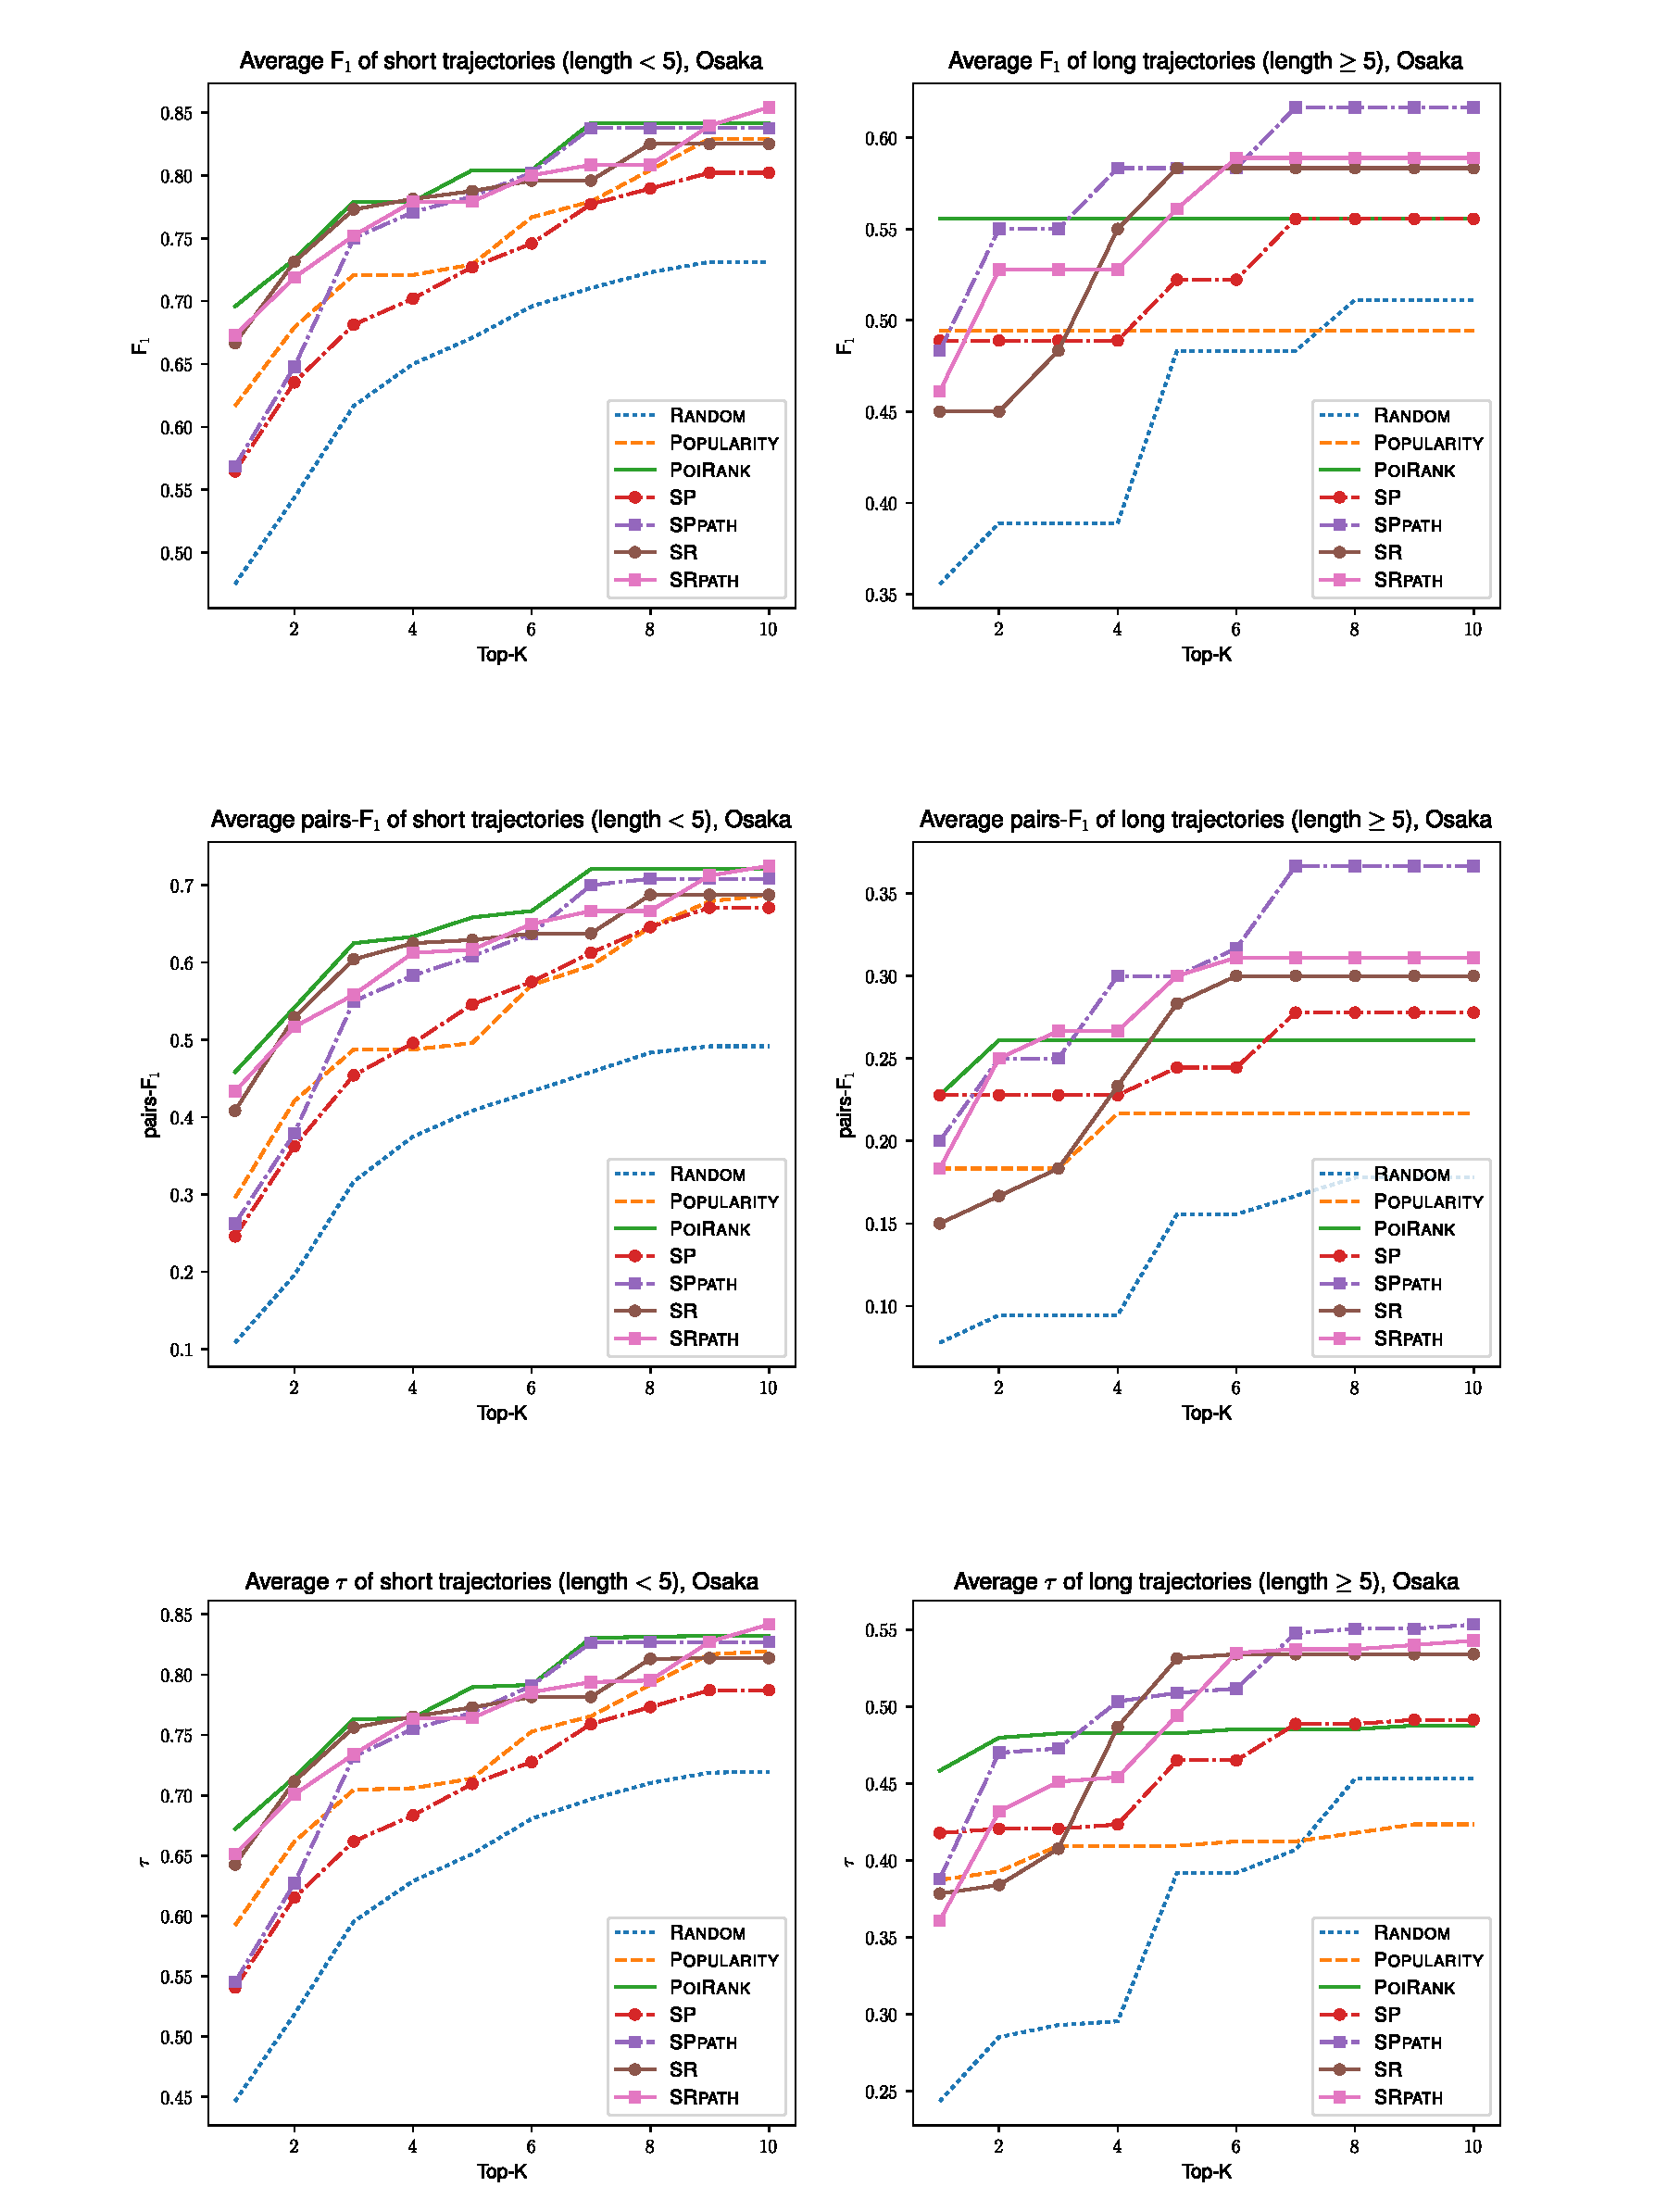
\includepdf[pages={1,2,4}]{plot_topk.pdf}
